\section{Display}

När programmet startas visar displayen möjligheter att välja aktiv bana, om
gemensam målgång ska vara aktiverad, vilken varvtid bilarna ska hålla och
eventuellt hur många varv bilarna ska köra runt banan (exkluderat de fem
kalibreringsvarven). Se figur~\ref{fig:disp:before}.

Under körning ska displayen för varje bil visa den förra varvtiden, hur många
varv bilen kört, nuvarande hastighet och pålagd spänning. Användaren kan också
trycka på en knapp för att avbryta körningen. Se figur~\ref{fig:disp:during}. I
mån av tid ska displayen även visa en karta över bilbanan och var systemet tror
att bilarna befinner sig.

Efter körningen är avklarad ska displayen visa olika grafer. Enligt
kravspecifikationen ska varvtid per varv och \textbf{???} visas enligt
figur~\ref{fig:disp:after}. I mån av tid ska endast en graf åt gången visas på
skärmen och ska användaren kunna välja vilken graf som ska visas med hjälp av
tryckbara knappar längst upp på skärmen.

\afterpage{%
  \clearpage
  \begin{figure}
    \centering
    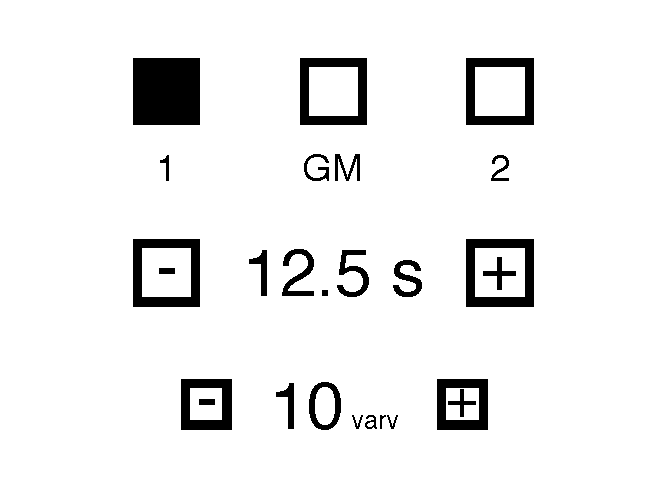
\includegraphics{innan}
    \caption{Displayens utseende vid val av körinställningar.}
    \label{fig:disp:before}
  \end{figure}
}
\afterpage{%
  \clearpage
  \begin{figure}
    \centering
    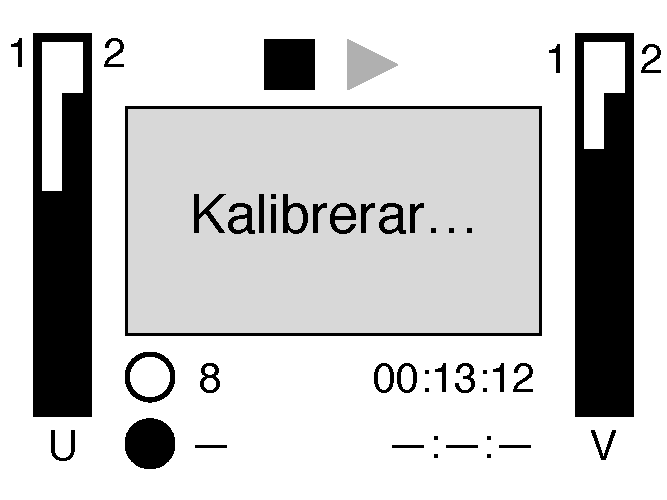
\includegraphics{under}
    \caption{Displayens utseende under körning.}
    \label{fig:disp:during}
  \end{figure}
}
